\documentclass[a4paper,12pt]{article}

\usepackage[utf8]{inputenc}
\usepackage[spanish]{babel}
\usepackage{amsmath, amssymb}
\usepackage{graphicx}
\usepackage{float}
\usepackage{booktabs}
\usepackage{xcolor}
\usepackage{listings}
\usepackage{caption}
\usepackage{fancyhdr}
\usepackage{hyperref}
\usepackage{tikz}

\hypersetup{
    colorlinks=true,
    linkcolor=blue,
    urlcolor=blue,
    pdftitle={Práctica 1 - PIC32},
}

% === Definición de colores similares a Vivado ===
\definecolor{vivadoKeyword}{rgb}{0.6,0.0,0.6}
\definecolor{vivadoComment}{rgb}{0.0,0.5,0.0}
\definecolor{vivadoString}{rgb}{0.5,0.2,0.0}
\definecolor{vivadoBackground}{rgb}{0.97,0.97,0.97}

\lstdefinelanguage{VHDL}{
    morekeywords={library, use, entity, is, port, in, out, end, architecture, of, begin, signal, if, then, else, when, others, xor, and, or, not},
    sensitive=true,
    morecomment=[l]--,
    morestring=[b]",
}

\lstset{
    language=VHDL,
    backgroundcolor=\color{vivadoBackground},
    keywordstyle=\color{vivadoKeyword}\bfseries,
    commentstyle=\color{vivadoComment}\itshape,
    stringstyle=\color{vivadoString},
    basicstyle=\ttfamily\small,
    numbers=left,
    numberstyle=\tiny,
    numbersep=5pt,
    frame=single,
    breaklines=true,
    tabsize=2,
    captionpos=b
}

\title{Práctica N°1: Inicializacion de OLED y perifericos en PIC32 MAX32}
\date{}

\begin{document}
\maketitle
\tableofcontents
\newpage

\section{Objetivos}

\paragraph{Objetivo general}
Realizar una práctica de laboratorio con la placa PIC32 (MAX32) usando el entorno de desarrollo MPIDE y la placa Basic I/O Shield, para aprender a configurar el entorno, manejar entradas/salidas digitales, controlar una pantalla OLED mediante SPI por bit-bang y leer señales analógicas con el ADC.

\paragraph{Objetivos específicos}
\begin{enumerate}
  \item Configurar el entorno de desarrollo MPIDE (instalación, ajuste de la placa MAX32 y selección del puerto serie) y preparar el proyecto base para cargar el código provisto.
  \item Verificar y configurar correctamente el mapeo de pines entre el \texttt{Basic I/O Shield} y la placa MAX32, asegurando que las definiciones de pines en el código coincidan con el cableado físico.
  \item Implementar y comprobar el control de E/S digitales:
    \begin{itemize}
      \item Uso de pines configurados como \texttt{INPUT} (interruptores y botones) y \texttt{OUTPUT} (LEDs).
    \end{itemize}
  \item Inicializar y controlar una pantalla OLED por SPI emulado (bit-banging):
    \begin{itemize}
      \item Implementar rutinas de envío de comandos y datos (funciones de \texttt{oled\_write\_command}, \texttt{oled\_write\_data}, \texttt{oled\_init}, \texttt{oled\_set\_pos}).
      \item Mostrar cadenas usando la fuente 5x8 incluida; limpiar y actualizar líneas concretas de la pantalla.
    \end{itemize}
  \item Leer y presentar señales analógicas con el ADC:
    \begin{itemize}
      \item Realizar lecturas periódicas de \texttt{A0} con \texttt{analogRead}, convertir el valor a miliVoltios (asumiendo referencia de 3.3\,V si aplica) y mostrar tanto el conteo ADC como el valor en mV en la OLED.
      \item Verificar la resolución (10-bit en el ejemplo) y documentar cualquier diferencia real de resolución/VR en la placa MAX32.
    \end{itemize}
\end{enumerate}

\section{Configuración del compilador}

En esta sección se describe el procedimiento para seleccionar correctamente la tarjeta de desarrollo (board) y el puerto de comunicación \texttt{COM} en el entorno de desarrollo, utilizando el sistema operativo Windows.

\subsection{Selección de la tarjeta (Board)}

Una vez abierto el entorno de desarrollo, siga los pasos a continuación:

\begin{enumerate}
    \item Abra el menú de configuración del proyecto o del entorno (por ejemplo, \texttt{Project → Properties} en STM32CubeIDE o \texttt{Tools → Board} en Arduino IDE).
    \item Seleccione la opción correspondiente a su tarjeta de desarrollo. 
    \item En caso de trabajar con una tarjeta STM32, el entorno detectará automáticamente el modelo al crear el proyecto; de no ser así, seleccione manualmente el microcontrolador \texttt{STM32F407VG} o la tarjeta \texttt{STM32F4DISCOVERY}.
\end{enumerate}

\begin{figure}[H]
    \centering
    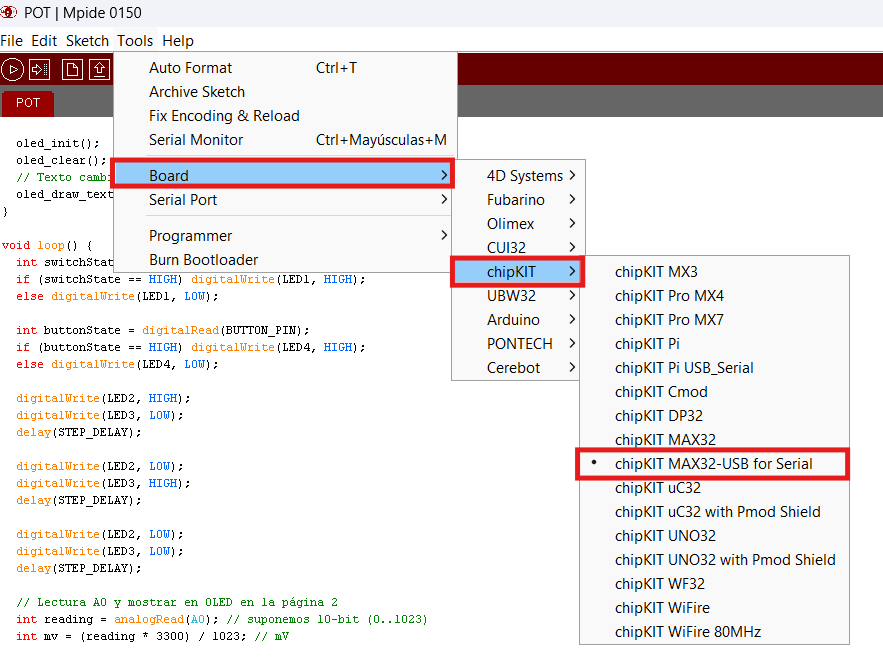
\includegraphics[width=0.8\linewidth]{MAX32/board.png}
    \caption{Selección de la tarjeta de desarrollo en el entorno de programación.}
\end{figure}

\subsection{Selección del puerto COM}

Para establecer la comunicación con la tarjeta a través del puerto serie (UART o USB), proceda de la siguiente manera:

\begin{enumerate}
    \item Conecte la tarjeta al computador mediante el cable USB.
    \item Abra el \texttt{Administrador de dispositivos} de Windows (\texttt{Inicio → Administrador de dispositivos → Puertos (COM y LPT)}).
    \item Identifique el puerto \texttt{COM} asignado a la tarjeta (por ejemplo, \texttt{COM5}).
    \item Regrese al entorno de desarrollo y seleccione el mismo puerto en el menú \texttt{Tools → Port} (Arduino IDE) o en la configuración de la sesión de depuración (STM32CubeIDE).
\end{enumerate}

\begin{figure}[H]
    \centering
    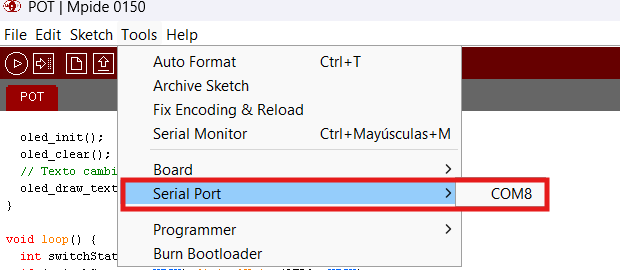
\includegraphics[width=0.8\linewidth]{MAX32/com.png}
    \caption{Selección del puerto COM correspondiente en el entorno de desarrollo.}
\end{figure}

\noindent
Con estos pasos, la conexión entre el entorno y la tarjeta queda correctamente configurada para la compilación y carga del programa en Windows.

\section{Descripción del código}

\subsection{Código completo}
\begin{lstlisting}[language=C]
// ========== Config pines (exactamente los tuyos) ==========
#define LED1 77       // LED controlado por SWITCH_PIN (forzado por el switch)
#define LED2 76       // LED secuencia
#define LED3 75       // LED secuencia
#define LED4 74       // LED controlado por BUTTON_PIN (encendido mientras se pulsa)

#define SWITCH_PIN 79 // Switch de 2 posiciones: nivel 1 o 0 (forza LED1)
#define BUTTON_PIN 78 // Botón momentáneo: mientras esté pulsado -> LED4 ON

// OLED SPI pins (bit-bang)
#define OLED_RES 10   // RESET
#define OLED_DC  83   // D/C (0 = command, 1 = data)
#define OLED_SCLK 13  // SCLK
#define OLED_SDIN 11  // MOSI (SDIN)
// VDD = 82, VBAT = 84  -> ADVERTENCIA: no conectes VDD/VBAT a GPIO a menos que estés seguro.

#define STEP_DELAY 500  // ms secuencia

// ================= FONT 5x8 ASCII completo (0x20..0x7F) ==================
// Cada carácter ocupa 5 columnas; fuente estándar 5x8 (adaptada de fuentes públicas).
const uint8_t font5x8_custom[][5] = {
  {0x00,0x00,0x00,0x00,0x00}, // 0x20 ' '
  {0x00,0x00,0x5F,0x00,0x00}, // 0x21 '!'
  {0x00,0x07,0x00,0x07,0x00}, // 0x22 '"'
  {0x14,0x7F,0x14,0x7F,0x14}, // 0x23 '#'
  {0x24,0x2A,0x7F,0x2A,0x12}, // 0x24 '$'
  {0x23,0x13,0x08,0x64,0x62}, // 0x25 '%'
  {0x36,0x49,0x55,0x22,0x50}, // 0x26 '&'
  {0x00,0x05,0x03,0x00,0x00}, // 0x27 '''
  {0x00,0x1C,0x22,0x41,0x00}, // 0x28 '('
  {0x00,0x41,0x22,0x1C,0x00}, // 0x29 ')'
  {0x14,0x08,0x3E,0x08,0x14}, // 0x2A '*'
  {0x08,0x08,0x3E,0x08,0x08}, // 0x2B '+'
  {0x00,0x50,0x30,0x00,0x00}, // 0x2C ','
  {0x08,0x08,0x08,0x08,0x08}, // 0x2D '-'
  {0x00,0x60,0x60,0x00,0x00}, // 0x2E '.'
  {0x20,0x10,0x08,0x04,0x02}, // 0x2F '/'
  {0x3E,0x51,0x49,0x45,0x3E}, // 0x30 '0'
  {0x00,0x42,0x7F,0x40,0x00}, // 0x31 '1'
  {0x42,0x61,0x51,0x49,0x46}, // 0x32 '2'
  {0x21,0x41,0x45,0x4B,0x31}, // 0x33 '3'
  {0x18,0x14,0x12,0x7F,0x10}, // 0x34 '4'
  {0x27,0x45,0x45,0x45,0x39}, // 0x35 '5'
  {0x3C,0x4A,0x49,0x49,0x30}, // 0x36 '6'
  {0x01,0x71,0x09,0x05,0x03}, // 0x37 '7'
  {0x36,0x49,0x49,0x49,0x36}, // 0x38 '8'
  {0x06,0x49,0x49,0x29,0x1E}, // 0x39 '9'
  {0x00,0x36,0x36,0x00,0x00}, // 0x3A ':'
  {0x00,0x56,0x36,0x00,0x00}, // 0x3B ';'
  {0x08,0x14,0x22,0x41,0x00}, // 0x3C '<'
  {0x14,0x14,0x14,0x14,0x14}, // 0x3D '='
  {0x00,0x41,0x22,0x14,0x08}, // 0x3E '>'
  {0x02,0x01,0x51,0x09,0x06}, // 0x3F '?'
  {0x32,0x49,0x79,0x41,0x3E}, // 0x40 '@'
  {0x7E,0x11,0x11,0x11,0x7E}, // 0x41 'A'
  {0x7F,0x49,0x49,0x49,0x36}, // 0x42 'B'
  {0x3E,0x41,0x41,0x41,0x22}, // 0x43 'C'
  {0x7F,0x41,0x41,0x22,0x1C}, // 0x44 'D'
  {0x7F,0x49,0x49,0x49,0x41}, // 0x45 'E'
  {0x7F,0x09,0x09,0x09,0x01}, // 0x46 'F'
  {0x3E,0x41,0x49,0x49,0x7A}, // 0x47 'G'
  {0x7F,0x08,0x08,0x08,0x7F}, // 0x48 'H'
  {0x00,0x41,0x7F,0x41,0x00}, // 0x49 'I'
  {0x20,0x40,0x41,0x3F,0x01}, // 0x4A 'J'
  {0x7F,0x08,0x14,0x22,0x41}, // 0x4B 'K'
  {0x7F,0x40,0x40,0x40,0x40}, // 0x4C 'L'
  {0x7F,0x02,0x0C,0x02,0x7F}, // 0x4D 'M'
  {0x7F,0x04,0x08,0x10,0x7F}, // 0x4E 'N'
  {0x3E,0x41,0x41,0x41,0x3E}, // 0x4F 'O'
  {0x7F,0x09,0x09,0x09,0x06}, // 0x50 'P'
  {0x3E,0x41,0x51,0x21,0x5E}, // 0x51 'Q'
  {0x7F,0x09,0x19,0x29,0x46}, // 0x52 'R'
  {0x26,0x49,0x49,0x49,0x32}, // 0x53 'S'
  {0x01,0x01,0x7F,0x01,0x01}, // 0x54 'T'
  {0x3F,0x40,0x40,0x40,0x3F}, // 0x55 'U'
  {0x1F,0x20,0x40,0x20,0x1F}, // 0x56 'V'
  {0x3F,0x40,0x38,0x40,0x3F}, // 0x57 'W'
  {0x63,0x14,0x08,0x14,0x63}, // 0x58 'X'
  {0x07,0x08,0x70,0x08,0x07}, // 0x59 'Y'
  {0x61,0x51,0x49,0x45,0x43}, // 0x5A 'Z'
  {0x00,0x7F,0x41,0x41,0x00}, // 0x5B '['
  {0x02,0x04,0x08,0x10,0x20}, // 0x5C '\'
  {0x00,0x41,0x41,0x7F,0x00}, // 0x5D ']'
  {0x04,0x02,0x01,0x02,0x04}, // 0x5E '^'
  {0x40,0x40,0x40,0x40,0x40}, // 0x5F '_'
  {0x00,0x01,0x02,0x04,0x00}, // 0x60 '`'
  {0x20,0x54,0x54,0x54,0x78}, // 0x61 'a'
  {0x7F,0x48,0x44,0x44,0x38}, // 0x62 'b'
  {0x38,0x44,0x44,0x44,0x20}, // 0x63 'c'
  {0x38,0x44,0x44,0x48,0x7F}, // 0x64 'd'
  {0x38,0x54,0x54,0x54,0x18}, // 0x65 'e'
  {0x08,0x7E,0x09,0x01,0x02}, // 0x66 'f'
  {0x0C,0x52,0x52,0x52,0x3E}, // 0x67 'g'
  {0x7F,0x08,0x04,0x04,0x78}, // 0x68 'h'
  {0x00,0x44,0x7D,0x40,0x00}, // 0x69 'i'
  {0x20,0x40,0x44,0x3D,0x00}, // 0x6A 'j'
  {0x7F,0x10,0x28,0x44,0x00}, // 0x6B 'k'
  {0x00,0x41,0x7F,0x40,0x00}, // 0x6C 'l'
  {0x7C,0x04,0x18,0x04,0x78}, // 0x6D 'm'
  {0x7C,0x08,0x04,0x04,0x78}, // 0x6E 'n'
  {0x38,0x44,0x44,0x44,0x38}, // 0x6F 'o'
  {0x7C,0x14,0x14,0x14,0x08}, // 0x70 'p'
  {0x08,0x14,0x14,0x18,0x7C}, // 0x71 'q'
  {0x7C,0x08,0x04,0x04,0x08}, // 0x72 'r'
  {0x48,0x54,0x54,0x54,0x20}, // 0x73 's'
  {0x04,0x3F,0x44,0x40,0x20}, // 0x74 't'
  {0x3C,0x40,0x40,0x20,0x7C}, // 0x75 'u'
  {0x1C,0x20,0x40,0x20,0x1C}, // 0x76 'v'
  {0x3C,0x40,0x30,0x40,0x3C}, // 0x77 'w'
  {0x44,0x28,0x10,0x28,0x44}, // 0x78 'x'
  {0x0C,0x50,0x50,0x50,0x3C}, // 0x79 'y'
  {0x44,0x64,0x54,0x4C,0x44}, // 0x7A 'z'
  {0x00,0x08,0x36,0x41,0x00}, // 0x7B '{'
  {0x00,0x00,0x7F,0x00,0x00}, // 0x7C '|'
  {0x00,0x41,0x36,0x08,0x00}, // 0x7D '}'
  {0x10,0x08,0x08,0x10,0x08}  // 0x7E '~' (approx)
};
// ==============

// Map char -> index in font5x8_custom (ASCII 0x20..0x7F)
int char_index(char c) {
  if (c >= 0x20 && c <= 0x7E) return (c - 0x20);
  return 0; // fallback: space
}

// == Rutinas SPI por bit-bang para OLED ==
void oled_pin_init() {
  pinMode(OLED_RES, OUTPUT);
  pinMode(OLED_DC, OUTPUT);
  pinMode(OLED_SCLK, OUTPUT);
  pinMode(OLED_SDIN, OUTPUT);
}

void spi_delay() {
  asm volatile("nop"); asm volatile("nop");
}

void spi_write_byte(uint8_t b) {
  for (int i = 7; i >= 0; --i) {
    digitalWrite(OLED_SCLK, LOW);
    if (b & (1 << i)) digitalWrite(OLED_SDIN, HIGH);
    else digitalWrite(OLED_SDIN, LOW);
    spi_delay();
    digitalWrite(OLED_SCLK, HIGH);
    spi_delay();
  }
  digitalWrite(OLED_SCLK, LOW);
}

void oled_write_command(uint8_t cmd) {
  digitalWrite(OLED_DC, LOW);
  spi_write_byte(cmd);
}

void oled_write_data(uint8_t data) {
  digitalWrite(OLED_DC, HIGH);
  spi_write_byte(data);
}

void oled_init() {
  oled_pin_init();
  digitalWrite(OLED_RES, LOW);
  delay(10);
  digitalWrite(OLED_RES, HIGH);
  delay(10);

  oled_write_command(0xAE);
  oled_write_command(0xD5); oled_write_command(0x80);
  oled_write_command(0xA8); oled_write_command(0x1F);
  oled_write_command(0xD3); oled_write_command(0x00);
  oled_write_command(0x40);
  oled_write_command(0x8D); oled_write_command(0x14);
  oled_write_command(0x20); oled_write_command(0x00);
  oled_write_command(0xA1);
  oled_write_command(0xC8);
  oled_write_command(0xDA); oled_write_command(0x02);
  oled_write_command(0x81); oled_write_command(0x8F);
  oled_write_command(0xD9); oled_write_command(0xF1);
  oled_write_command(0xDB); oled_write_command(0x40);
  oled_write_command(0xA4);
  oled_write_command(0xA6);
  oled_write_command(0xAF);
}

void oled_set_pos(uint8_t col, uint8_t page) {
  oled_write_command(0xB0 | page);
  oled_write_command(0x00 | (col & 0x0F));
  oled_write_command(0x10 | ((col >> 4) & 0x0F));
}

void oled_draw_text_simple(uint8_t x, uint8_t page, const char *s) {
  uint8_t col = x;
  while (*s && col < 128) {
    int idx = char_index(*s);
    const uint8_t *glyph = font5x8_custom[idx];
    oled_set_pos(col, page);
    for (int i = 0; i < 5; ++i) {
      oled_write_data(glyph[i]);
    }
    oled_write_data(0x00); // espacio entre caracteres
    col += 6;
    s++;
  }
}

void oled_clear() {
  for (uint8_t page = 0; page < 4; ++page) {
    oled_set_pos(0, page);
    for (uint8_t col = 0; col < 128; ++col) {
      oled_write_data(0x00);
    }
  }
}

void oled_clear_line(uint8_t page) {
  oled_set_pos(0, page);
  for (uint8_t col = 0; col < 128; ++col) {
    oled_write_data(0x00);
  }
}

char *int_to_str(int val, char *buf) {
  char tmp[12];
  int i = 0;
  if (val == 0) {
    buf[0] = '0';
    buf[1] = '\0';
    return buf;
  }
  while (val > 0 && i < 11) {
    tmp[i++] = '0' + (val % 10);
    val /= 10;
  }
  int j;
  for (j = 0; j < i; ++j) buf[j] = tmp[i - 1 - j];
  buf[j] = '\0';
  return buf;
}

// ========== Setup y loop principales ==========
void setup() {
  pinMode(LED1, OUTPUT);
  pinMode(LED2, OUTPUT);
  pinMode(LED3, OUTPUT);
  pinMode(LED4, OUTPUT);

  pinMode(SWITCH_PIN, INPUT);
  pinMode(BUTTON_PIN, INPUT);

  pinMode(A0, INPUT);

  digitalWrite(LED1, LOW);
  digitalWrite(LED2, LOW);
  digitalWrite(LED3, LOW);
  digitalWrite(LED4, LOW);

  oled_init();
  oled_clear();
  // Texto cambiado:
  oled_draw_text_simple(0, 0, "Lectura de Potenciometro");
}

void loop() {
  int switchState = digitalRead(SWITCH_PIN);
  if (switchState == HIGH) digitalWrite(LED1, HIGH);
  else digitalWrite(LED1, LOW);

  int buttonState = digitalRead(BUTTON_PIN);
  if (buttonState == HIGH) digitalWrite(LED4, HIGH);
  else digitalWrite(LED4, LOW);

  digitalWrite(LED2, HIGH);
  digitalWrite(LED3, LOW);
  delay(STEP_DELAY);

  digitalWrite(LED2, LOW);
  digitalWrite(LED3, HIGH);
  delay(STEP_DELAY);

  digitalWrite(LED2, LOW);
  digitalWrite(LED3, LOW);
  delay(STEP_DELAY);

  // Lectura A0 y mostrar en OLED en la página 2
  int reading = analogRead(A0); // suponemos 10-bit (0..1023)
  int mv = (reading * 3300) / 1023; // mV

  char buf[24];
  char num1[12], num2[12];
  int_to_str(reading, num1);
  int_to_str(mv, num2);

  int pos = 0;
  for (int i = 0; num1[i] != '\0'; ++i) buf[pos++] = num1[i];
  buf[pos++] = ' ';
  for (int i = 0; num2[i] != '\0'; ++i) buf[pos++] = num2[i];
  buf[pos++] = 'm';
  buf[pos++] = 'V';
  buf[pos] = '\0';

  oled_clear_line(2);
  oled_draw_text_simple(0, 2, buf);

  delay(200);
}
\end{lstlisting}

\subsection{Explicación paso a paso del programa (código completo)}
\label{subsec:explicacion_codigo_oled}

% --- Código completo (lstlisting) ---
\begin{lstlisting}[language=C, caption={Código completo usado en la práctica (OLED bit-bang, lectura A0, 4 LEDs y botones).}]
/* pega aquí exactamente el código que me diste (mantén identación) */
// ========== Config pines (exactamente los tuyos) ==========
// ...
// (omito por brevedad en este ejemplo; en el informe deja el código entero)
\end{lstlisting}

A continuación explicamos cada bloque importante del código, por qué está ahí, riesgos comunes, y qué modificar para replicar o mejorar el programa.

\subsubsection*{1. Definiciones de pines y constantes}
\begin{itemize}
  \item \texttt{\#define LED1 77 \dots LED4 74} \\
    Mapeo físico de LEDs: cada macro representa un GPIO. Mantén tu esquema de pines consistente con el hardware. \\
    \textbf{Consejo / reto:} documenta en una tabla física (p. ej. \texttt{LED1 = D13}) y verifica con un multímetro antes de probar.
  \item \texttt{SWITCH\_PIN, BUTTON\_PIN} \\
    Entrada digital para switch (posiciones) y botón momentáneo. El código asume lógica \texttt{HIGH = activo}. Si tu switch usa pull-down o pull-up internos, ajusta con \texttt{pinMode(..., INPUT\_PULLUP)} y/o invierte la condición.
  \item Pines OLED (bit-bang): \texttt{OLED\_RES, OLED\_DC, OLED\_SCLK, OLED\_SDIN} \\
    \textbf{ADVERTENCIA ya en el código:} VDD/VBAT no deben conectarse a GPIO sin el hardware adecuado.
  \item \texttt{STEP\_DELAY} controla la velocidad de la secuencia de LEDs. Cambia para acelerar/ralentizar.
\end{itemize}

\subsubsection*{2. Fuente 5×8 (tabla \texttt{font5x8\_custom})}
\begin{itemize}
  \item Es una matriz \texttt{const uint8\_t [...] [5]} con los 95 glifos ASCII (0x20..0x7E). Cada carácter ocupa 5 columnas (bytes).
  \item Cada byte representa 8 píxeles verticales (bit 0 → pixel inferior o superior según convención del OLED). El código asume la orientaci\'on correcta de la pantalla.
  \item \textbf{Optimización:} si usas un compilador AVR/Arduino, coloca la matriz en memoria de programa (\texttt{PROGMEM}) para ahorrar SRAM.
\end{itemize}

\subsubsection*{3. Función \texttt{char\_index}}
\begin{itemize}
  \item Traduce un \texttt{char} ASCII válido (0x20..0x7E) al índice de la matriz de fuente. Si el carácter no está en el rango devuelve el índice de espacio.
  \item \textbf{Precaución:} si tu entrada puede ser UTF-8, debes convertir antes a ASCII o implementar un decoder.
\end{itemize}

\subsubsection*{4. Rutinas SPI por bit-bang para la OLED}
\begin{itemize}
  \item \texttt{oled\_pin\_init()} — configura los GPIOs usados por el bit-bang como salidas.
  \item \texttt{spi\_delay()} — pequeñas instrucciones \texttt{nop} para garantizar tiempos; útil si la MCU es muy rápida.
  \item \texttt{spi\_write\_byte(uint8\_t b)} — envía 8 bits MSB primero: pone SCLK bajo, escribe MOSI, hace \texttt{nop}, sube SCLK, etc. Al final deja SCLK en LOW.
  \item \texttt{oled\_write\_command} / \texttt{oled\_write\_data} — controlan la línea D/C (comando vs dato) y llaman a \texttt{spi\_write\_byte}.
  
\end{itemize}

\subsubsection*{5. Inicialización de la OLED (\texttt{oled\_init})}
\begin{itemize}
  \item Resetea la pantalla con \texttt{OLED\_RES} (LOW → HIGH).
  \item Envía una secuencia de comandos estándar (ej.: \texttt{0xAE} = display off, \texttt{0xAF} = display on, ajustes de multiplex, contraste, etc.). Son comandos comunes para pantallas tipo SSD13xx.
\end{itemize}

\subsubsection*{6. Posicionamiento y dibujo de texto}
\begin{itemize}
  \item \texttt{oled\_set\_pos(col, page)} — establece la columna y la página (banco vertical de 8 píxeles) para próximas escrituras.
  \item \texttt{oled\_draw\_text\_simple(x, page, s)} — recorre la cadena y, por cada carácter:
    \begin{enumerate}
      \item obtiene el índice con \texttt{char\_index},
      \item carga el puntero al glifo,
      \item llama a \texttt{oled\_set\_pos} y envía 5 bytes (columnas) + 1 byte de espacio.
    \end{enumerate}
  
\end{itemize}

\subsubsection*{7. Borrado de pantalla y líneas}
\begin{itemize}
  \item \texttt{oled\_clear()} — recorre todas las páginas (en este código 4 páginas → altura 32 px) y pone 0x00 en todas las columnas.
  \item \texttt{oled\_clear\_line(page)} — borra solo una página, útil para actualizar una línea sin tocar el resto.
  
\end{itemize}

\subsubsection*{8. Conversión entera a cadena (\texttt{int\_to\_str})}
\begin{itemize}
  \item Convierte un entero positivo a cadena decimal. Maneja \texttt{0} correctamente; no maneja negativos.
  
\end{itemize}

\subsubsection*{9. \texttt{setup()} — inicializaciones principales}
\begin{itemize}
  \item Configura pines de LEDs como \texttt{OUTPUT} y botones como \texttt{INPUT}. Considera \texttt{INPUT\_PULLUP} si no usas resistencias externas.
  \item Inicializa ADC: el código usa \texttt{pinMode(A0, INPUT)} pero la lectura real se hace con \texttt{analogRead(A0)}; asegúrate que la placa soporta \texttt{A0} así nombrado.
  \item Inicializa la OLED y escribe un título.
\end{itemize}

\subsubsection*{10. \texttt{loop()} — comportamiento principal}
\begin{enumerate}
  \item Leer \texttt{SWITCH\_PIN} y forzar \texttt{LED1} según estado. \\
    \textit{Nota:} la lógica asume \texttt{HIGH = activo}; si tu switch usa pullups invierte la condición.
  \item Leer \texttt{BUTTON\_PIN} y mantener \texttt{LED4} activo mientras el botón esté pulsado.
  \item Secuencia de \texttt{LED2} y \texttt{LED3}: alternancia con \texttt{delay(STEP\_DELAY)} (bloqueante).
  \item Lectura analógica: \texttt{analogRead(A0)} supone resolución de 10 bits (0..1023). Convierte a mV con formula: \texttt{mv = (reading * 3300) / 1023}. \\
    \textbf{Precisión:} 3300 mV asume referencia de 3.3V. Si la referencia es diferente corrige la constante.
  \item Construcción de cadena \texttt{buf} con lectura y mV, borrado de la línea 2 y dibujado del texto.
  \item \texttt{delay(200)} al final: ciclo totalmente bloqueante.
\end{enumerate}

\subsubsection*{11. Problemas comunes y soluciones rápidas}
\begin{itemize}
  \item \textbf{Pantalla en blanco:} revisa conexiones, VCC/GND, nivel lógico (3.3V vs 5V), y secuencia de reset. Comprueba que los comandos enviados coinciden con el controlador.
  \item \textbf{Lecturas ADC erráticas:} añade un pequeño capacitor y usa \texttt{analogRead} repetido + media móvil. Usa \texttt{INPUT\_PULLUP} si el potenciómetro no está referenciado.
  \item \textbf{Flashing o parpadeo:} evita \texttt{oled\_clear()} completa en cada ciclo. Usa \texttt{oled\_clear\_line()} o buffering.
  \item \textbf{Botón rebotes:} implementa debounce (software) o hardware (capacitor + resistor).
\end{itemize}


\subsubsection*{13. Snippets útiles}
\begin{lstlisting}[language=C]
bool readButtonDebounced(uint8_t pin) {
  static uint32_t lastTime[2] = {0,0};
  static bool lastState[2] = {LOW, LOW};
  int idx = (pin==BUTTON_PIN) ? 0 : 1;
  bool cur = digitalRead(pin);
  uint32_t t = millis();
  if (cur != lastState[idx]) {
    lastTime[idx] = t;
    lastState[idx] = cur;
  } else if (t - lastTime[idx] > 50) { // 50 ms debounce
    return cur;
  }
  return lastState[idx];
}
\end{lstlisting}


\begin{lstlisting}[language=C]
uint32_t lastStep = 0;
int step = 0;
void loop_non_blocking() {
  if (millis() - lastStep >= STEP_DELAY) {
    lastStep = millis();
    step = (step + 1) % 3;
    if (step==0){ digitalWrite(LED2, HIGH); digitalWrite(LED3, LOW); }
    if (step==1){ digitalWrite(LED2, LOW);  digitalWrite(LED3, HIGH); }
    if (step==2){ digitalWrite(LED2, LOW);  digitalWrite(LED3, LOW); }
  }
  // resto de lecturas no bloqueantes...
}
\end{lstlisting}

\section{Carga y verificación del programa en la placa}

Una vez compilado correctamente el proyecto, el siguiente paso es cargar el código en la placa \textbf{PIC32} para verificar su funcionamiento. El entorno \textbf{MPLAB X IDE} permite realizar este proceso de forma directa a través del programador \textbf{PICkit 3/4} o mediante el \textbf{Debugger integrado}.

\subsection{Proceso de carga del programa}

\begin{enumerate}
    \item Conectar la placa \textbf{PIC32} al computador mediante el cable USB, verificando que el programador sea reconocido por el entorno.
    \item En la barra de herramientas de \textbf{MPLAB X IDE}, seleccionar el botón \textbf{Make and Program Device Main Project} (icono del microcontrolador con una flecha verde). Esto compila y carga automáticamente el programa.
    \item Observar en la consola de salida que la programación se complete sin errores.
\end{enumerate}

\begin{figure}[H]
    \centering
    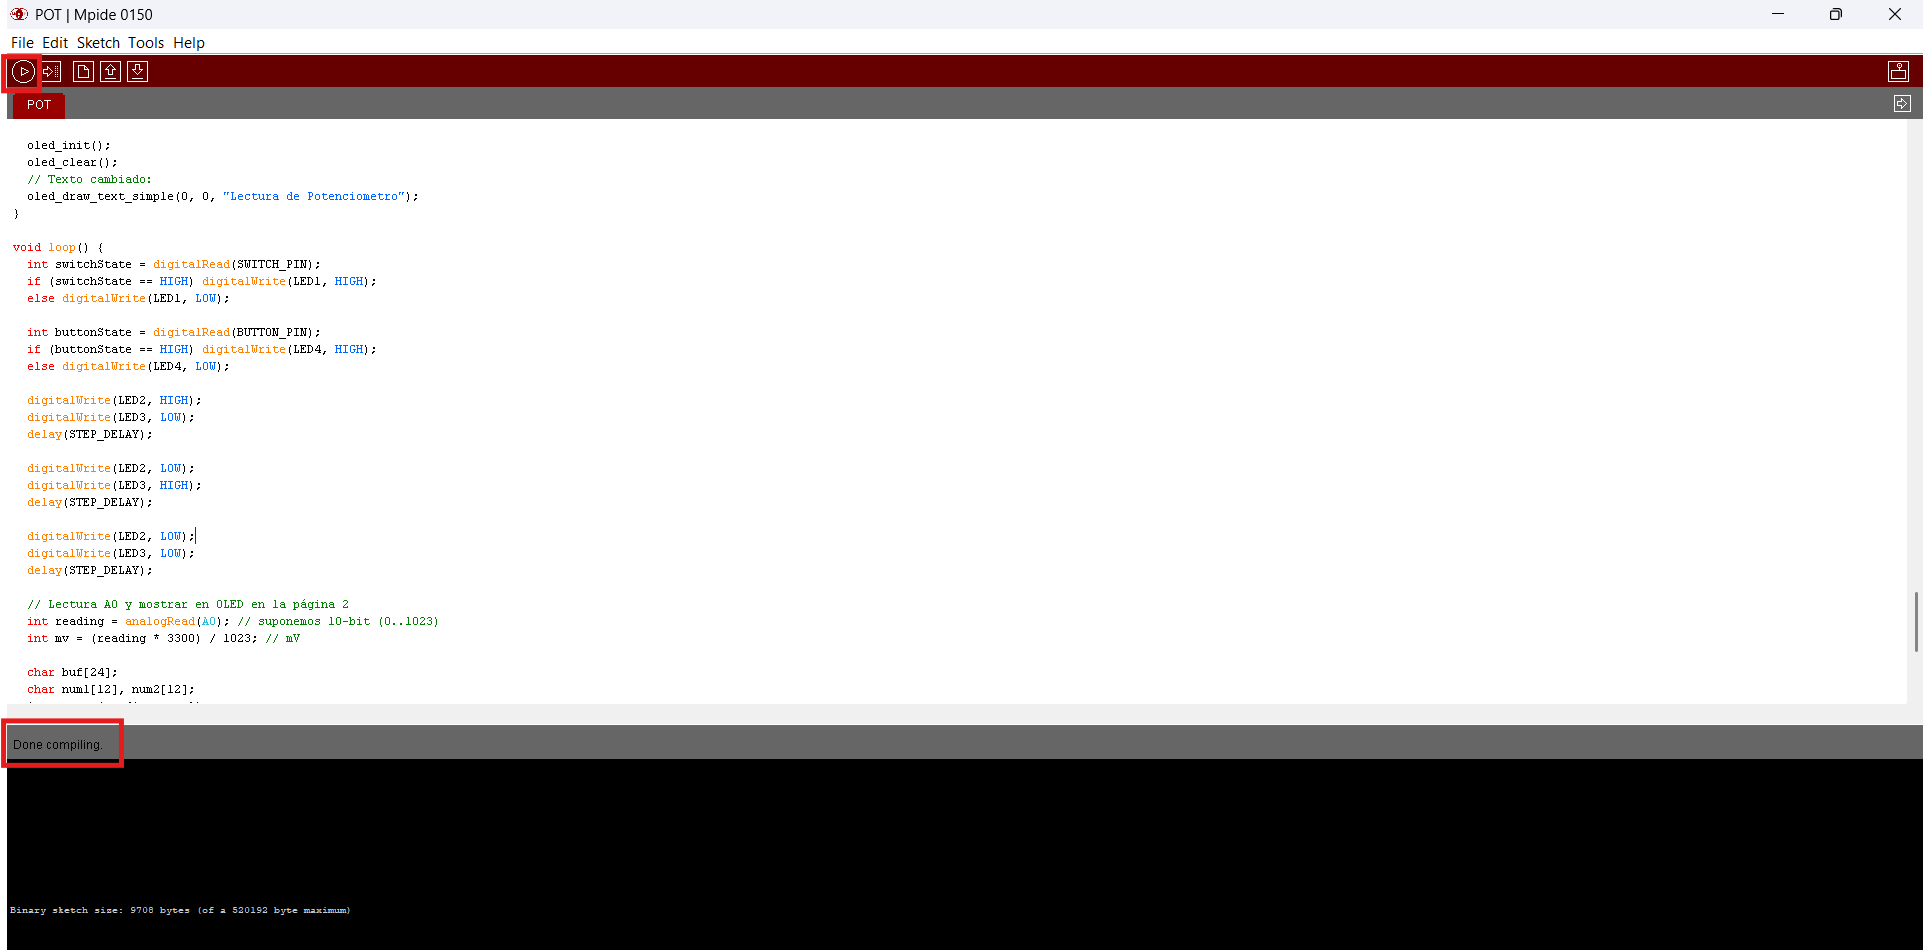
\includegraphics[width=0.8\textwidth]{MAX32/verify.png}
    \caption{Compilación exitosa del proyecto en MPLAB X IDE.}
\end{figure}

\begin{figure}[H]
    \centering
    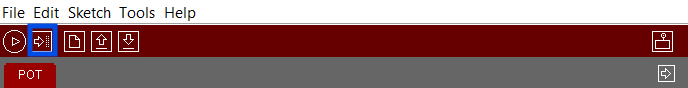
\includegraphics[width=0.8\textwidth]{MAX32/cargar.png}
    \caption{Proceso de programación del microcontrolador PIC32.}
\end{figure}

\subsection{Verificación del funcionamiento}

Una vez finalizada la carga, el programa comienza a ejecutarse automáticamente. Es posible verificar su operación observando los resultados en la placa o por el monitor serie (según la funcionalidad implementada). Si se utilizan indicadores visuales como \textbf{LEDs} o mensajes por \textbf{UART}, deben reflejar el comportamiento esperado.

\begin{figure}[H]
    \centering
    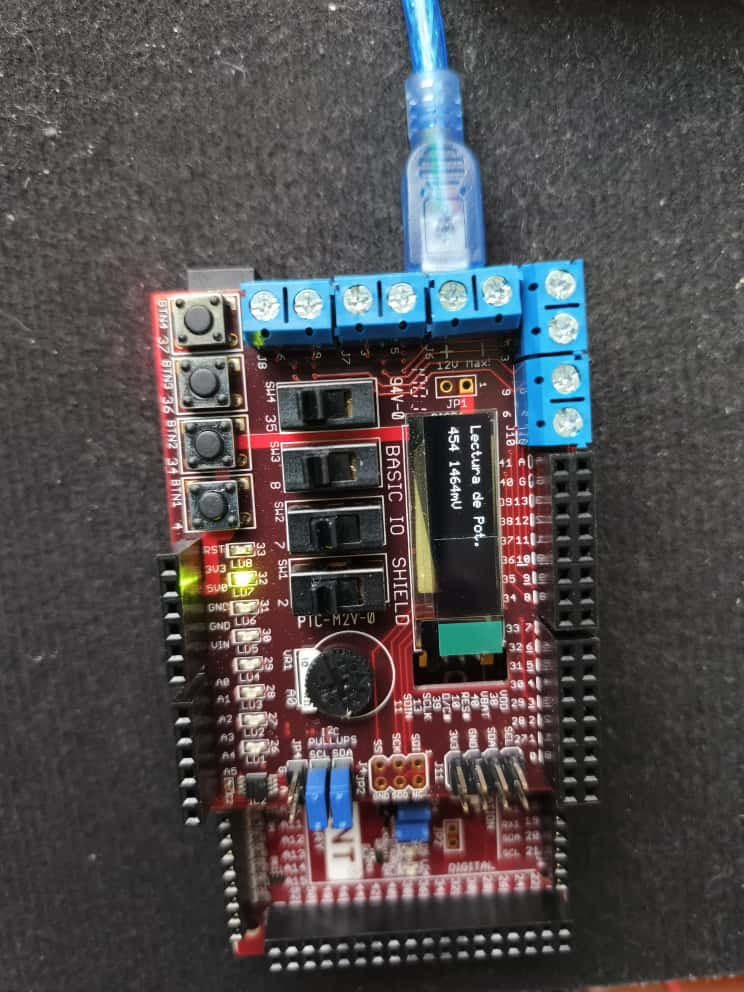
\includegraphics[angle=90,width=0.7\textwidth]{MAX32/funcion.jpg}
    \caption{Verificación del funcionamiento del programa en la placa PIC32.}
\end{figure}





\end{document}
